% Compile with
% lualatex filename.tex
% biber filename.bcf
% lualatex filename.tex
% lualatex filename.tex
% or just using:
% make

\documentclass[
  uofacolor,
  BCOR=12mm,     % 12mm binding corrections
  %parskip=half,  % new paragraphs start with half line vertical space
  open=odd,      % chapter start on odd and even pages
  cleardoublepage=plain,
  DIV=15
]{uofathesis}


% Warning, if another latex run is needed
\usepackage[aux]{rerunfilecheck}

% just list chapters, sections and subsections in the toc
% change to 1 if you only want chapters and sections
\setcounter{tocdepth}{2}

% no space after new paragraph
\setlength\parindent{0pt}

%------------------------------------------------------------------------------
%------------------------------ Language and Font: --------------------------
%------------------------------------------------------------------------------
\usepackage{fontspec}
\defaultfontfeatures{Ligatures=TeX}  % -- becomes en-dash etc.

% language
\usepackage{polyglossia}
\setmainlanguage[variant=british]{english}

% intelligent quotation marks, language and nesting sensitive
\usepackage[autostyle]{csquotes}

% microtypographical features, makes the text look nicer on the small scale
\usepackage{microtype}

% for checkmark
\usepackage{wasysym}

% for fonts
\setsansfont[Scale=MatchLowercase]{Gill Sans SemiBold}
\setmainfont{Palatino}
\newfontfamily\myfont{Gill Sans}


%------------------------------------------------------------------------------
%------------------------ For Math Environment --------------------------------
%------------------------------------------------------------------------------

\usepackage{amsmath}
\usepackage{amssymb}
\usepackage{mathtools}

% Enable Unicode-Math and follow the ISO-Standards for typesetting math
\usepackage[
  math-style=ISO,
  bold-style=ISO,
  sans-style=italic,
  nabla=upright,
  partial=upright,
]{unicode-math}
\setmathfont{Latin Modern Math}

% nice, small fracs for the text with \sfrac{}{}
\usepackage{xfrac}  


%------------------------------------------------------------------------------
%---------------------------- Numbers and Units -------------------------------
%------------------------------------------------------------------------------

\usepackage[
  locale=US,
  separate-uncertainty=true,
  per-mode=symbol-or-fraction,
]{siunitx}
\sisetup{math-micro=\text{µ},text-micro=µ}

%------------------------------------------------------------------------------
%-------------------------------- tables  -------------------------------------
%------------------------------------------------------------------------------

\usepackage{booktabs}       % provides \toprule, \midrule, \bottomrule
\usepackage{xtab}

%------------------------------------------------------------------------------
%-------------------------------- graphics -------------------------------------
%------------------------------------------------------------------------------

\usepackage{graphicx}
\usepackage{grffile}

% allow figures to be placed in the running text by default:
\usepackage{scrhack}
\usepackage{float}
\floatplacement{figure}{htbp}
\floatplacement{table}{htbp}

% keep figures and tables in the section
\usepackage[section, below]{placeins}

% figures in text
\usepackage{wrapfig}



%------------------------------------------------------------------------------
%---------------------- customize list environments ---------------------------
%------------------------------------------------------------------------------

\usepackage{enumitem}

%------------------------------------------------------------------------------
%------------------------------ Bibliograpy ---------------------------------
%------------------------------------------------------------------------------

\usepackage[
  backend=biber,   % use modern biber backend
  autolang=hyphen, % load hyphenation rules
  natbib=true,
  style=authoryear,
  maxbibnames=5,
  maxcitenames=2,
  uniquelist=false,
  url=false, 
  doi=false,
  isbn=false,
  eprint=false                
]{biblatex}

% include the bibliography
\addbibresource{bib/ref_author.bib} 
\addbibresource{bib/ref_physics.bib} 
\setlength{\bibitemsep}{\baselineskip}

%------------------------------------------------------------------------------
%------------------------------ Others: ------------------------------------
%------------------------------------------------------------------------------

\usepackage[hidelinks, pdfusetitle,unicode,linkbordercolor=uofadarkblue, citecolor=uofadarkblue, urlcolor=uofadarkblue]{hyperref}
\usepackage{bookmark}
\usepackage[shortcuts]{extdash}

\usepackage{listings}
\lstset{ %
  basicstyle=\footnotesize\ttfamily, 
  language=C
}

% for lorem ipsum
\usepackage{blindtext}


\usepackage[rightcaption]{sidecap}
\sidecaptionvpos{figure}{c}

% command to allow "appendix A.1" instead of "section A.1" with autoref
\newcommand{\aref}[1]{\hyperref[#1]{Appendix~\ref{#1}}}

% commands to color citations, without changing contents to only one color
\let\oldcite=\cite
\renewcommand{\cite}[1]{\textcolor{uofadarkblue}{\oldcite{#1}}}
\let\oldcitep=\citep
\renewcommand{\citep}[1]{\textcolor{uofadarkblue}{\oldcitep{#1}}}

\usepackage[nolist, nohyperlinks]{acronym}



%------------------------------------------------------------------------------
%-------------------------    Thesis Information   ----------------------------
%------------------------------------------------------------------------------

% Information for title page
\author{\myfont{Albert Einstein}}
\title{\Huge The Main Title of the Thesis}
\subtitle{\LARGE The Subtitle of the Thesis}
\date{\myfont{October 2018}}
\thesisclass{Honours}

\school{School of Physical Sciences}
\faculty{Faculty of Sciences}
\department{Department of Physics}
\university{The University of Adelaide}

% Information for second page
\submissiondate{10th October 2018}
\firstadvisor{Prof.~Dr.~John Doe}
\secondadvisor{Prof.~Dr.~Jane Doe}

% UofA logo on top of the titlepage
\titlehead{\includegraphics[height=3cm, trim={0.5cm 0 0 0},clip]{logos/UofA.jpg}}

\begin{document}

\frontmatter

\maketitle

\makeadvisorpage

% general front pages, numbered in Roman numerals
\thispagestyle{plain}
\section*{Abstract}

The abstract must not exceed 500 words. \newline
It could be structured as follows: Motivation and aim of the thesis, methods, results.

\vspace{0.1cm}

\blindtext[3]


% choose if / which originality declaration you need to add
\cleardoublepage
\thispagestyle{empty}
\section*{Declaration of Originality}

I certify that this work contains no material which has been accepted for the award of any other degree or diploma in my name in any university or other tertiary institution and, to the best of my knowledge and belief, contains no material previously published or written by another person, except where due reference has been made in the text. 
In addition, I certify that no part of this work will, in the future, be used in a submission in my name for any other degree or diploma in any university or other tertiary institution without the prior approval of the University of Adelaide and where applicable, any partner institution responsible for the joint award of this degree.

I give consent to this copy of my thesis, when deposited in the University Library, being made available for loan and photocopying, subject to the provisions of the Copyright~Act~1968.

I also give permission for the digital version of my thesis to be made available on the web, via the University's digital research repository, the Library Search and also through web search engines, unless permission has been granted by the University to restrict access for a period of time.

%Add the following paragraph ONLY if you are a Research Training Program (RTP) funded student:
%I acknowledge the support I have received for my research through the provision of an Australian Government Research Training Program Scholarship.

\vspace*{1cm}\noindent
\begin{center}
\begin{tabular}{@{}p{0.4\textwidth}@{\hspace{0.15\textwidth}}p{0.4\textwidth}@{}}
\rule{\linewidth}{0.25pt}& \rule{\linewidth}{0.25pt}\\
Date & Signature
\end{tabular}
\end{center}
\input{./content/00_originality_publications.tex}
\cleardoublepage
\thispagestyle{empty}
\section*{Acknowledgment}

\blindtext[4]

\tableofcontents

%%%%%%%%%%%%%%
\newcommand{\p}[1]{\textcolor{uofadarkblue}{\texttt{#1}}}
%%%%%%%%%%%%%

\mainmatter

% actual thesis, starting with page 1 in arabic numbers
\chapter{Introduction}

\begin{flushright}
	\textit{Space is big. Really big.\\You just won't believe how vastly, hugely, mind-bogglingly big it is.}

	\vspace{0.3cm}
	--- Douglas Adams, \textit{The Hitchhiker's Guide to the Galaxy}
	\vspace{0.3cm}
\end{flushright}

How big is big? 
Hundreds of thousands of years are already necessary for light to traverse our Galaxy, comprising hundreds of billions of stars.
The Universe is even bigger with 2 trillion of similar galaxies accessible to our observations.
The size of the observable universe has been determined by the Planck space mission to be 13.8 billion light years, deduced from the most precise map of the cosmic microwave background to date.
This is already vastly big, but the Universe beyond the observable one is once again by a multitude bigger.
Arthur Dent -- the main character in \textit{The Hitchhiker's Guide to the Galaxy} -- must have felt rather lost in this mind-bogglingly big space.

\vspace{0.2cm}

\blindtext[3]

\clearpage

\blindtext[1]

\vspace{0.2cm}

This thesis deals with ...
 
\vspace{0.2cm}

For these purposes, the thesis is structured as follows:

\begin{description}[leftmargin=0cm]
\item[\textcolor{uofablue}{Chapter 2}] gives an overview of ...
\item[\textcolor{uofablue}{Chapter 3}] explains ...
\item[\textcolor{uofablue}{Chapter 4}] describes ...
\item[\textcolor{uofablue}{Chapter 5}] presents ...
\item[\textcolor{uofablue}{Chapter 6}] illustrates ...
\end{description}

\chapter{Astroparticle Physics at a Glance}

\begin{flushright}
    \textit{All you really need to know for the moment \\is that the Universe is a lot more complicated than you might think, \\even if you start from a position of thinking it’s pretty damn complicated in the first place.}

    \vspace{0.3cm}
    --- Douglas Adams, \textit{The Hitchhiker's Guide to the Galaxy}
    \vspace{0.3cm}
\end{flushright}

%
\begin{figure}
    \centering
    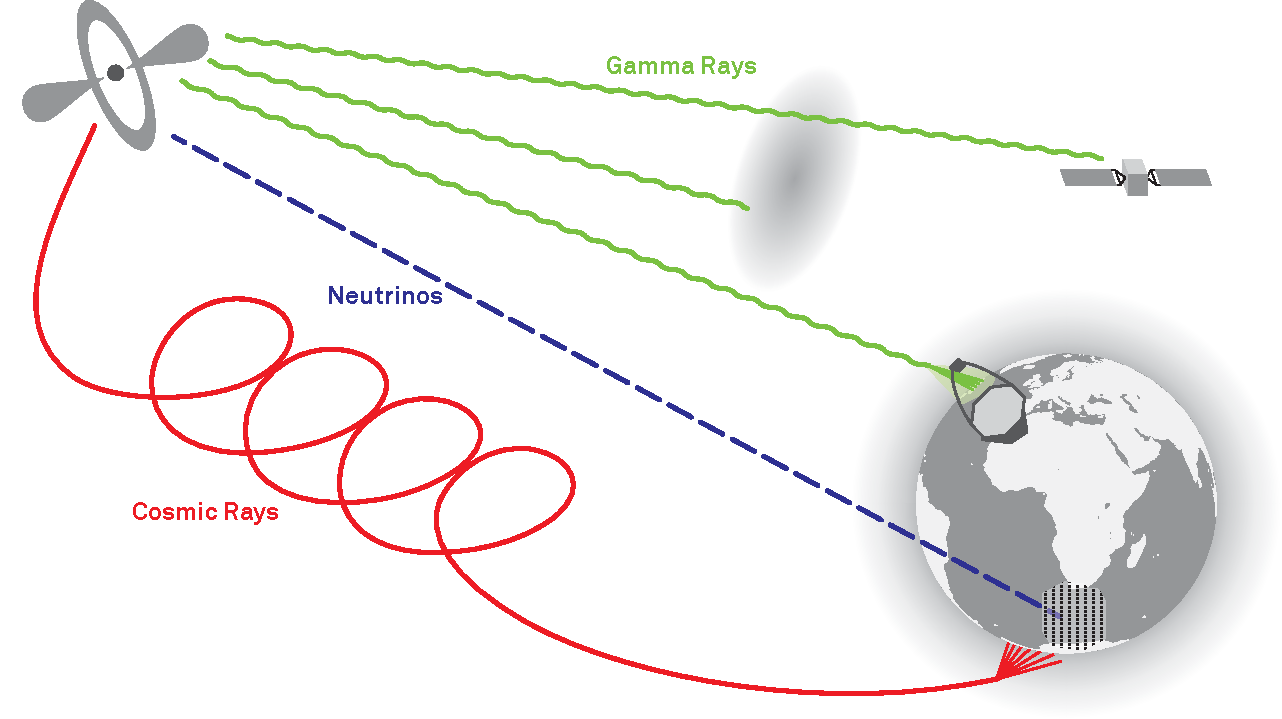
\includegraphics[width=0.9\textwidth]{./figures/agn_earth_messenger.pdf}
    \caption{Astroparticle physics at a glance. Specific astronomical objects emit different messengers, such as neutrinos, cosmic and gamma rays, propagating through the universe. Depending on the type of messenger, they might interact with magnetic fields, interstellar clouds, the Earth's atmosphere or the Earth itself, and they can be detected with different instruments.}
    \label{fig:overview_astro}
\end{figure}
%

\blindtext[4]



\chapter{Tipps}


\section{References}
\label{sec:references}

The use of \texttt{autoref} from the \texttt{hyperref} package is really useful.
It automatically writes the type, e.\,g.\ Figure, section, subsection, of your reference.
Like this, not only the number of your reference, but also the type is used for the link.
Furthermore, no linebreaks between the type and the number will occur.
To use it, just replace \texttt{\textbackslash ref} by \texttt{\textbackslash autoref}.

Here is an example to show the differences between the commands:
\ref{sec:references} vs.\ \autoref{sec:references}.

For the appendix, the use of \texttt{\textbackslash autoref} will create the following:

\autoref{app:magic} for the chapter, and \autoref{sec:selected_data} for the section.
For sections, you might want to have it differently.
Therefore, a specific command has been added in the preamble.
Just use \texttt{\textbackslash aref} instead of \texttt{\textbackslash autoref}, and you will get the following:

\aref{sec:selected_data} for the section.


\section{Citations}

The adavantage of using the citationstyle author year (instead of numbers or abbreviations) is that a reader from your field will most probably know the corresponding publication and will not need to check the bibliography.
Moreover, a name is easier to remember than just a number.
Therefore, you will make it easier for the reader to read your thesis (and you want to make it as comfortable for your referee as possible).

In principle, there are two situations where you want to cite something:
\texttt{\textbackslash cite}: \cite{malaga} suggests to use model XY.
\texttt{\textbackslash citep}: The model describes the formation of stars  \citep{malaga}.


\section{Graphics}

\section{Tables}

\section{Structure of the Thesis}


% Start of appendix, numbered in latin letters
\appendix
\chapter{Multi-Wavelength Analysis}

%%%%%%%%%%%%%%%%%%%%%%%%%%%%%%%%%%%%%%%%%%%%%%%%%%%%%%%%%%%%%%%%%%%

\section{Coordinates of Associated Sources}

\begin{table}
\centering

\caption{Coordinates of associated 3FGL sources.}
\label{tab:assoc_coord}

\tiny

\begin{tabular}{l r c c}
\toprule
3FGL Name & Associated Name & RA & Dec \\
\midrule
3FGL J0001.2-0748  &  PMN J0001-0746  &  0.32512  &  -7.77417  \\
3FGL J0001.4+2120  &  TXS 2358+209  &  0.38488  &  21.22674  \\
3FGL J0002.2-4152  &  1RXS J000135.5-415519  &  0.39723  &  -41.91437  \\
3FGL J0003.2-5246  &  RBS 0006  &  0.83158  &  -52.79081  \\
3FGL J0003.8-1151  &  PMN J0004-1148  &  1.02048  &  -11.81622  \\
3FGL J0004.7-4740  &  PKS 0002-478  &  1.14856  &  -47.60545  \\
3FGL J0006.4+3825  &  S4 0003+38  &  1.48823  &  38.33754  \\
3FGL J0008.0+4713  &  MG4 J000800+4712  &  1.99988  &  47.20217  \\
3FGL J0008.6-2340  &  RBS 0016  &  2.1475  &  -23.65775  \\
3FGL J0009.1+0630  &  CRATES J000903.95+062821.5  &  2.26646  &  6.47264  \\
3FGL J0009.3+5030  &  NVSS J000922+503028  &  2.34388  &  50.50803  \\
3FGL J0009.6-3211  &  IC 1531  &  2.39824  &  -32.27701  \\
3FGL J0012.4+7040  &  TXS 0008+704  &  2.88293  &  70.75878  \\
3FGL J0013.2-3954  &  PKS 0010-401  &  3.24962  &  -39.90724  \\
3FGL J0013.9-1853  &  RBS 0030  &  3.48354  &  -18.9019  \\
3FGL J0014.0-5025  &  RBS 0032  &  3.54675  &  -50.37572  \\
3FGL J0014.6+6119  &  4C +60.01  &  3.7033  &  61.29543  \\
3FGL J0014.7+5802  &  1RXS J001442.2+580201  &  3.67546  &  58.0337  \\
3FGL J0015.7+5552  &  GB6 J0015+5551  &  3.91729  &  55.86242  \\
3FGL J0016.3-0013  &  S3 0013-00  &  4.0462  &  -0.25346  \\
3FGL J0017.2-0643  &  PMN J0017-0650  &  4.28908  &  -6.84264  \\
3FGL J0017.6-0512  &  PMN J0017-0512  &  4.39924  &  -5.2116  \\
3FGL J0018.4+2947  &  RBS 0042  &  4.61562  &  29.79178  \\
3FGL J0018.9-8152  &  PMN J0019-8152  &  4.83596  &  -81.881  \\
3FGL J0019.1-5645  &  PMN J0019-5641  &  4.86071  &  -56.69525  \\
3FGL J0019.4+2021  &  PKS 0017+200  &  4.90773  &  20.36268  \\
3FGL J0021.6-6835  &  PKS 0021-686  &  6.02792  &  -68.3485  \\
3FGL J0021.6-2553  &  CRATES J002132.55-255049.3  &  5.38563  &  -25.84703  \\
3FGL J0022.1-1855  &  1RXS J002209.2-185333  &  5.53862  &  -18.89303  \\
3FGL J0022.1-5141  &  1RXS J002159.2-514028  &  5.50025  &  -51.67344  \\
3FGL J0022.5+0608  &  PKS 0019+058  &  5.63517  &  6.13452  \\
3FGL J0023.5+4454  &  B3 0020+446  &  5.89768  &  44.94327  \\
3FGL J0024.4+0350  &  GB6 J0024+0349  &  6.188333  &  3.817639  \\
3FGL J0026.7-4603  &  1RXS J002636.3-460101  &  6.64879  &  -46.01922  \\
3FGL J0028.6+7507  &  GB6 J0028+7506  &  7.05479  &  75.10372  \\
3FGL J0028.8+1951  &  TXS 0025+197  &  7.12424  &  20.00743  \\
3FGL J0029.1-7045  &  PKS 0026-710  &  7.17312  &  -70.75447  \\
3FGL J0030.2-1646  &  1RXS J003019.6-164723  &  7.58167  &  -16.78972  \\
3FGL J0030.3-4223  &  PKS 0027-426  &  7.57327  &  -42.41278  \\
3FGL J0030.7-0209  &  PKS B0027-024  &  7.6326  &  -2.19893  \\
3FGL J0031.3+0724  &  NVSS J003119+072456  &  7.83217  &  7.41578  \\
3FGL J0032.3-2852  &  PMN J0032-2849  &  8.13792  &  -28.82231  \\
3FGL J0033.6-1921  &  KUV 00311-1938  &  8.3925  &  -19.35925  \\
3FGL J0035.2+1513  &  RX J0035.2+1515  &  8.81135  &  15.25115  \\
3FGL J0035.9+5949  &  1ES 0033+595  &  8.96935  &  59.83461  \\
3FGL J0037.9+1239  &  NVSS J003750+123818  &  9.46187  &  12.63856  \\
3FGL J0038.0-2501  &  PKS 0035-252  &  9.5614  &  -24.98395  \\
3FGL J0038.0+0012  &  NVSS J003808+001336  &  9.53543  &  0.22682  \\
3FGL J0039.0-2218  &  PMN J0039-2220  &  9.78421  &  -22.33372  \\
3FGL J0039.1-0939  &  TXS 0036-099  &  9.77622  &  -9.71302  \\
3FGL J0039.1+4330  &  NVSS J003907+433015  &  9.78296  &  43.50431  \\
3FGL J0040.3+4049  &  B3 0037+405  &  10.0575  &  40.83464  \\
3FGL J0040.5-2339  &  PMN J0040-2340  &  10.10379  &  -23.66689  \\
3FGL J0041.9+3639  &  RX J0042.0+3641  &  10.535  &  36.6875  \\
3FGL J0042.0+2318  &  PKS 0039+230  &  10.51894  &  23.33363  \\
3FGL J0043.5-0444  &  1RXS J004333.7-044257  &  10.89217  &  -4.71681  \\
3FGL J0043.7-1117  &  1RXS J004349.3-111612  &  10.95288  &  -11.26867  \\
3FGL J0043.8+3425  &  GB6 J0043+3426  &  10.95353  &  34.44059  \\
\bottomrule
\end{tabular}
\end{table}


\begin{table} \ContinuedFloat
\centering
\caption{-- continued from previous page}
\tiny

\begin{tabular}{l r c c}
\toprule
3FGL Name & Associated Name & RA & Dec \\
\midrule
3FGL J0045.2-3704  &  PKS 0042-373  &  11.30025  &  -37.09667  \\
3FGL J0045.3+2126  &  GB6 J0045+2127  &  11.33042  &  21.46114  \\
3FGL J0045.7+1217  &  GB6 J0045+1217  &  11.43059  &  12.28661  \\
3FGL J0046.7-8419  &  PKS 0044-84  &  11.11192  &  -84.37781  \\
3FGL J0047.0+5658  &  GB6 J0047+5657  &  11.75179  &  56.96178  \\
3FGL J0047.9+5447  &  1RXS J004754.5+544758  &  11.96608  &  54.79581  \\
3FGL J0048.0+3950  &  B3 0045+395  &  11.98008  &  39.816  \\
3FGL J0048.0+2236  &  NVSS J004802+223525  &  12.01092  &  22.59006  \\
3FGL J0049.4-5401  &  PMN J0049-5402  &  12.45354  &  -54.04536  \\
3FGL J0049.4-4149  &  1RXS J004939.9-415133  &  12.41625  &  -41.85917  \\
3FGL J0049.7+0237  &  PKS 0047+023  &  12.43015  &  2.61772  \\
3FGL J0049.8-5737  &  PKS 0047-579  &  12.4978  &  -57.64093  \\
3FGL J0050.0-4458  &  PMN J0049-4457  &  12.31933  &  -44.95319  \\
3FGL J0050.4-0449  &  PKS 0047-051  &  12.58973  &  -4.87239  \\
3FGL J0050.6-0929  &  PKS 0048-09  &  12.67216  &  -9.48478  \\
3FGL J0051.0-0649  &  PKS 0048-071  &  12.78421  &  -6.83395  \\
3FGL J0051.2-6241  &  1RXS J005117.7-624154  &  12.81942  &  -62.70117  \\
3FGL J0054.8-2455  &  FRBA J0054-2455  &  13.69471  &  -24.92486  \\
3FGL J0055.2-1213  &  TXS 0052-125  &  13.79909  &  -12.29919  \\
3FGL J0056.3-2116  &  PMN J0056-2117  &  14.1345  &  -21.28556  \\
3FGL J0056.3-0935  &  TXS 0053-098  &  14.08367  &  -9.60831  \\
3FGL J0057.9-0542  &  PKS 0055-059  &  14.52111  &  -5.66452  \\
3FGL J0058.0-3233  &  PKS 0055-328  &  14.50929  &  -32.57243  \\
3FGL J0058.3+3315  &  MG3 J005830+3311  &  14.63362  &  33.18812  \\
3FGL J0059.1-5701  &  PKS 0056-572  &  14.69409  &  -56.98652  \\
3FGL J0059.2-0152  &  1RXS J005916.3-015030  &  14.82054  &  -1.83822  \\
3FGL J0059.6+0003  &  PKS 0056-00  &  14.77298  &  0.11434  \\
3FGL J0100.2+0745  &  GB6 J0100+0745  &  15.08662  &  7.76428  \\
3FGL J0102.3+4217  &  GB6 J0102+4214  &  15.61313  &  42.23861  \\
3FGL J0102.8+5825  &  TXS 0059+581  &  15.69068  &  58.40309  \\
3FGL J0103.4+5336  &  1RXS J010325.9+533721  &  15.85817  &  53.62036  \\
3FGL J0103.7+1323  &  NVSS J010345+132346  &  15.94079  &  13.39614  \\
3FGL J0105.1-2415  &  PKS 0102-245  &  16.24252  &  -24.27457  \\
3FGL J0105.3+3928  &  GB6 J0105+3928  &  16.28833  &  39.47092  \\
3FGL J0107.0-1208  &  PMN J0107-1211  &  16.79913  &  -12.18989  \\
3FGL J0108.5-0035  &  PKS 0105-008  &  17.11184  &  -0.62338  \\
3FGL J0108.7+0134  &  4C +01.02  &  17.16155  &  1.58342  \\
3FGL J0109.1+1816  &  MG1 J010908+1816  &  17.28408  &  18.26875  \\
3FGL J0109.8+6132  &  TXS 0106+612  &  17.4431  &  61.55846  \\
3FGL J0109.9-4020  &  RBS 0158  &  17.48575  &  -40.34753  \\
3FGL J0110.2+6806  &  4C +67.04  &  17.55364  &  68.09478  \\
3FGL J0110.9-1254  &  1RXS J011050.0-125455  &  17.70838  &  -12.91769  \\
3FGL J0111.5+0535  &  1RXS J011130.5+053612  &  17.87579  &  5.6075  \\
3FGL J0112.1+2245  &  S2 0109+22  &  18.02427  &  22.74411  \\
3FGL J0112.8+3207  &  4C +31.03  &  18.20972  &  32.13818  \\
3FGL J0113.0-3554  &  PMN J0113-3551  &  18.31604  &  -35.86331  \\
3FGL J0113.4+4948  &  S4 0110+49  &  18.36253  &  49.80668  \\
3FGL J0114.8+1326  &  GB6 J0114+1325  &  18.71991  &  13.42708  \\
3FGL J0115.7+0356  &  PMN J0115+0356  &  18.9188  &  3.9454  \\
3FGL J0115.8+2519  &  RX J0115.7+2519  &  18.942375  &  25.3315  \\
3FGL J0116.0-1134  &  PKS 0113-118  &  19.05217  &  -11.60429  \\
3FGL J0116.2-2744  &  1RXS J011555.6-274428  &  18.98117  &  -27.74219  \\
3FGL J0116.3-6153  &  SUMSS J011619-615343  &  19.08117  &  -61.8955  \\
3FGL J0117.8-2113  &  PKS 0115-214  &  19.45325  &  -21.18518  \\
3FGL J0118.8-2142  &  PKS 0116-219  &  19.73859  &  -21.69171  \\
3FGL J0118.9-1457  &  1RXS J011905.4-145906  &  19.76925  &  -14.98292  \\
3FGL J0120.4-2700  &  PKS 0118-272  &  20.13193  &  -27.02351  \\
3FGL J0121.7+5154  &  NVSS J012133+515557  &  20.39025  &  51.93261  \\
3FGL J0122.8+3423  &  1ES 0120+340  &  20.78599  &  34.34685  \\
3FGL J0123.7-2312  &  1RXS J012338.2-231100  &  20.90996  &  -23.18292  \\
3FGL J0125.2-0627  &  PMN J0124-0624  &  21.21033  &  -6.41719  \\
3FGL J0125.4-2548  &  PKS 0122-260  &  21.32849  &  -25.81789  \\
3FGL J0126.1-2227  &  PKS 0123-226  &  21.56251  &  -22.376  \\
3FGL J0127.1-0818  &  PMN J0127-0821  &  21.81796  &  -8.35806  \\
3FGL J0127.2+0325  &  NVSS J012713+032259  &  21.80805  &  3.38353  \\
3FGL J0127.9+2551  &  4C +25.05  &  21.6783  &  25.98369  \\
3FGL J0128.5+4430  &  GB6 J0128+4439  &  22.17224  &  44.655  \\
3FGL J0130.8+1441  &  4C +14.06  &  22.48061  &  14.77995  \\
3FGL J0131.2+6120  &  1RXS J013106.4+612035  &  22.78028  &  61.34267  \\
3FGL J0131.3+5548  &  TXS 0128+554  &  22.80758  &  55.75364  \\
3FGL J0132.5-0802  &  PKS 0130-083  &  23.17136  &  -8.06801  \\
3FGL J0132.6-1655  &  PKS 0130-17  &  23.1812  &  -16.91348  \\
3FGL J0133.0-4413  &  SUMSS J013306-441422  &  23.27679  &  -44.23958  \\
3FGL J0133.2-5159  &  PKS 0131-522  &  23.27401  &  -52.0011  \\
3FGL J0133.3+4324  &  B3 0129+431  &  23.18386  &  43.42574  \\
3FGL J0134.3-3842  &  PMN J0134-3843  &  23.63346  &  -38.72594  \\
3FGL J0134.5+2638  &  1RXS J013427.2+263846  &  23.61792  &  26.64583  \\
3FGL J0135.0+6927  &  TXS 0130+691  &  23.66984  &  69.41969  \\
3FGL J0136.5+3905  &  B3 0133+388  &  24.13542  &  39.09989  \\
3FGL J0137.0+4752  &  OC 457  &  24.24414  &  47.85808  \\
3FGL J0137.6-2430  &  PKS 0135-247  &  24.409853  &  -24.514971  \\
3FGL J0137.8+5813  &  1RXS J013748.0+581422  &  24.46025  &  58.23644  \\
3FGL J0139.9+8735  &  NVSS J013913+873754  &  24.80571  &  87.63186  \\
3FGL J0141.4-0929  &  PKS 0139-09  &  25.35763  &  -9.4788  \\
3FGL J0143.7-5845  &  SUMSS J014347-584550  &  25.94842  &  -58.76394  \\
\bottomrule
\end{tabular}
\end{table}



\chapter{MAGIC Analysis}
\label{app:magic}

\section{Selected Data}
\label{sec:selected_data}

\subsection*{3FGLJ2346.7+0705 Data}

The following runs have been used for the MAGIC analysis of the source 3FGLJ2346.7+0705 and have been downloaded on superstar level:

\texttt{05055339, 05055340, 05055436, 05055437, 05055438, 05055439, 05055440, 05055441, 05055471, 05055472, 05055473, 05055474, 05055475, 05055502, 05055503, 05055504, 05055505, 05055506, 05055507, 05055581, 05055582, 05055583, 05055584, 05055629, 05055630, 05055631, 05055632, 05055633, 05055634, 05055635, 05055659, 05055660, 05055670, 05055671, 05055672, 05055699, 05055700, 05057801, 05057802, 05057803, 05057804, 05057838, 05057840, 05057895, 05058673, 05058855, 05058856, 05058857, 05058859.}

\vspace{0.3cm}

Additionally, the following subruns have been used for the MAGIC analysis of the source 3FGLJ2346.7+0705 and have been downloaded on star level:

\texttt{M1: 05057839.001-.020, 05057892.001-.005, .008-.011, .013, .015-.020, .022-.025, 05057893.001-.003, .005-.007, .009-.012, .014-.025, 05057894.001-.011, .013-.025, 05058674.001-.009, 05058858.001-.011, .016-.021.}

\texttt{M2: 05057839.001-.020, 05057892.001-.005, .008-.011, .013-.020, .022-.025, \newline05057893.001-.003, .005-.007, .010, .012, .015-.025, 05057894.001-.011, .013-.025, 05058674.001-.009, 05058858.001-.010, .015-.020.}



\subsection*{Crab Nebula Data}

The following runs have been used for the sanity check of the MAGIC analysis of the source 3FGLJ2346.7+0705 and for the Random Forest study, and have been downloaded on superstar level:

\texttt{05056516, 05056517, 05056587, 05056588, 05057065, 05057066, 05057067, 05057068, 05057069, 05057070, 05057144, 05057145, 05057146, 05057147, 05057148, 05057188, 05057189, 05057190, 05057191, 05057192, 05057649, 05057650, 05057651, 05057652, 05057653, 05057977, 05057978, 05058069, 05058072, 05058073, 05058074, 05058749, 05059266, 05059267, 05059268.}

\vspace{0.3cm}

Additionally, the following subruns have been used for the sanity check of the MAGIC analysis of the source 3FGLJ2346.7+0705 and the Random Forest study, and have been downloaded on star level:

\texttt{M1: 05057193.002-.004, 05059212.001-.012.}

\texttt{M2: 05057193.002-.004, 05059212.001-.012.}


\newpage


\subsection*{Data used as Hadrons}

The following runs have been used for the training of the gamma / hadron separation for the MAGIC analysis of the source 3FGLJ2346.7+0705 and have been downloaded on superstar level:

\texttt{1ES 0229+200: 05057396, 05057397, 05058048, 05058049, 05058461, 05058462, \newline 05058923, 05058924, 05058925, 05058926.}

\texttt{M15: 05055321, 05055322, 05055323, 05055324, 05055624, 05055625, 05055626, \newline 05056900, 05056901, 05056902, 05056903. }

\texttt{S3 0218+35: 05056153, 05056154, 05056155, 05056156, 05056617, 05056618, \newline 05057172, 05057173.}

\texttt{Triangulum II: 05055980, 05055981, 05056416, 05056417, 05057051, 05057052, \newline 05057865, 05057602, 05057603.}


\vspace{0.75cm}

The following runs have been used for the Random Forest study and have been downloaded on superstar level:

\texttt{1ES 0229+200: 05058048, 05058049, 05058461, 05058462, 05058925, 05058926.}

\texttt{M15: 05055321, 05055322, 05055625, 05055626, 05056900, 05056901. }

\texttt{S3 0218+35: 05056153, 05056154, 05056617, 05056618, 05057172, 05057173.}

\texttt{Triangulum II: 05056416, 05056417, 05057051, 05057052, 05057602, 05057603, \newline05057865.}

\newpage

%%%%%%%%%%%%%%%%%%%%%%%%%%%%%

\section{Input Cards}
\label{sec:input_cards}

\subsection*{coach.rc}

\begin{lstlisting}
RF.numTree:    100
RF.trainRatio: 0.95
RF.createTestSample: TRUE
RF.zdmin: 5.
RF.zdmax: 35.
RFLoop.FilterCuts.Continue0.Condition: MHillas_1.fSize<50. 
RFLoop.FilterCuts.Continue1.Condition: MHillas_2.fSize<50.
RFLoop.FilterCuts.Continue2.Condition: MHillas_1.fSize>50000. 
RFLoop.FilterCuts.Continue3.Condition: MHillas_2.fSize>50000. 
RFLoop.FilterCuts.Continue4.Condition: MNewImagePar_1.fLeakage1>0.15
RFLoop.FilterCuts.Continue5.Condition: MNewImagePar_2.fLeakage1>0.15 
RFLoop.FilterCuts.Continue6.Condition: MStereoPar.fValid<0.5

#####

RFLoop.GHCuts.Continue0.Condition: MImagePar_1.fNumIslands>1
RFLoop.GHCuts.Continue1.Condition: MImagePar_2.fNumIslands>1
RF.ReZenithing: TRUE
RF.numAzBins:   1
RF.numZdBins:   30
RF.NumTryGH: 3
RF.NdSizeGH: 5
RF.NumVariableGH: 12

RF.GHVariable1:  0.025+0.05*floor(log10(MHillas_1.fSize)/0.05)
RF.GHVariable2:  0.025+0.05*floor(log10(MHillas_2.fSize)/0.05)
RF.GHVariable3:  MHillas_1.fWidth
RF.GHVariable4:  MHillas_2.fWidth
RF.GHVariable5:  MHillas_1.fLength
RF.GHVariable6:  MHillas_2.fLength
RF.GHVariable7:  MStereoPar.fM1Impact
RF.GHVariable8:  MStereoPar.fM2Impact
RF.GHVariable9:  MStereoPar.fMaxHeight
RF.GHVariable10: sqrt(MHillasTimeFit_1.fP1Grad*MHillasTimeFit_1.fP1Grad)
RF.GHVariable11: sqrt(MHillasTimeFit_2.fP1Grad*MHillasTimeFit_2.fP1Grad)
RF.GHVariable12: (0.5/30.)+(1./30.)*floor(cos(MPointingPos_1.fZd*0.0174532925)/(1./30.))

#####

RFLoop.EnergyCuts.Continue0.Condition: MStereoPar.fCherenkovRadius<4000
RFLoop.EnergyCuts.Continue1.Condition: MStereoPar.fTheta2>0.1
RFLoop.EnergyCutsUnphys.Continue0.Condition: MStereoPar.fValid<1
RFLoop.EnergyCutsUnphys.Continue1.Condition: MStereoPar.fCherenkovDensity<0
MEnergyTable.SizeBinning 19
MEnergyTable.MinSize 25
MEnergyTable.MaxSize 200000
MEnergyTable.ImpactBinning 50
MEnergyTable.MinImpact 0
MEnergyTable.MaxImpact 3.5
MEnergyTable.ZdCorrectionFormula 0.97*pow(x,-0.3)/(1-pow(1-x,2.25))
MEnergyTable.LeakageCorrectionFormula_1 1-4*x*x
MEnergyTable.LeakageCut_1 0.2
MEnergyTable.LeakageCorrectionFormula_2 1-4*x*x
MEnergyTable.LeakageCut_2 0.2
MEnergyTable.BCorrectionFormula 0.93+0.2*sqrt(1.-pow(x,2))
MEnergyTable.MinEvtPerBin 3

########

RF.NumTryDisp: 3
RF.NdSizeDisp: 5
RF.NumVariableDisp: 11

RF.Disp1Variable1:  log10(MHillas_1.fSize)
RF.Disp1Variable2:  log10(MHillas_2.fSize)
RF.Disp1Variable3:  MStereoPar.fM1Impact
RF.Disp1Variable4:  MStereoPar.fM2Impact
RF.Disp1Variable5:  MPointingPos_1.fZd
RF.Disp1Variable6:  MStereoPar.fMaxHeight
RF.Disp1Variable7:  sqrt(MHillasTimeFit_1.fP1Grad*MHillasTimeFit_1.fP1Grad)
RF.Disp1Variable8:  sqrt(MHillasTimeFit_2.fP1Grad*MHillasTimeFit_2.fP1Grad)
RF.Disp1Variable9:  MHillas_1.fWidth
RF.Disp1Variable10: MHillas_1.fLength
# To be estimated in regression:
RF.Disp1Variable11: MHillasSrc_1.fDist*0.0033703

RF.Disp2Variable1:  log10(MHillas_1.fSize)
RF.Disp2Variable2:  log10(MHillas_2.fSize)
RF.Disp2Variable3:  MStereoPar.fM1Impact
RF.Disp2Variable4:  MStereoPar.fM2Impact
RF.Disp2Variable5:  MPointingPos_1.fZd
RF.Disp2Variable6:  MStereoPar.fMaxHeight
RF.Disp2Variable7:  sqrt(MHillasTimeFit_1.fP1Grad*MHillasTimeFit_1.fP1Grad)
RF.Disp2Variable8:  sqrt(MHillasTimeFit_2.fP1Grad*MHillasTimeFit_2.fP1Grad)
RF.Disp2Variable9:  MHillas_2.fWidth
RF.Disp2Variable10: MHillas_2.fLength
# To be estimated in regression:
RF.Disp2Variable11: MHillasSrc_2.fDist*0.0033703
\end{lstlisting}

\backmatter
\printbibliography

\end{document}
